\documentclass[12pt,a4paper]{amsart}
\usepackage[slovene]{babel}
\usepackage[utf8]{inputenc}
\usepackage{amsmath,amssymb,amsfonts}
\usepackage{url}
\usepackage[dvipsnames,usenames]{color}
\usepackage{graphicx}

\newcommand{\program}{FINANČNA MATEMATIKA}
\newcommand{\ime}{Brina Ribič, David Rozman}
\newcommand{\naslovdela}{Naključni sprehodi v grafih oblike lizike}
\newcommand{\letnica}{2022}

\begin{document}
    
\begin{center}
    \thispagestyle{empty}
\noindent{\large
UNIVERZA V LJUBLJANI\\[1mm]
FAKULTETA ZA MATEMATIKO IN FIZIKO\\[5mm]
\program\ -- 1.~stopnja}
\vfill
\end{center}


\begin{center}
{\bf \naslovdela}\\[10mm]
Kratek opis projekta\\[1cm]
\end{center}
\vfill

\begin{center}
    Avtorja: {\large
\ime}\\[2mm]
   \noindent{\large
Ljubljana, \letnica} 
\end{center}
\pagebreak

\section{Opis problema}

V projektni nalogi si bova natančneje ogledala naključne sprehode v grafih oblike lizike.
Za vhodni podatek bova vzela graf lizike, to je graf podan s parom $(m,n)$, 
kjer je $m$ število vozlišč, pri katerih ima graf obliko polnega grafa, 
$n$ pa je število vozlišč, na katerih ima graf obliko poti. Oba dela grafa sta povezana z mostom.
Naloga projekta je v takšnih grafih poiskati pričakovani čas, 
\begin{itemize}
    \item da obiščemo vsa vozlišča;
    \item da pridemo iz določenega vozlišča v drugega oziroma, da pridemo nazaj do začetnega vozlišča.
\end{itemize}
 Zanimalo naju bo tudi, kaj se zgodi s pričakovanimi časi, če graf lizike malo spremeniva - npr. 
 dodava poln graf na koncu poti ali ga dodava na začetek in konec poti.

\section{Matematično ozadje}

Naj bo $G = (V,E)$ graf lizike, kjer je $V = V(G)$ množica vozlišč in 
$E = E(G)$ množica povezav grafa $G$. Par $(m,n)$ pove, koliko vozlišč je pri delu grafa, ki ima obliko polnega grafa in
koliko jih je pri delu grafa, ki ima obliko poti, zaporedoma. Torej je skupno na grafu $m+n$ vozlišč 
in $\binom{m}{2} + n$ povezav.

% slika grafa
\begin{figure}[h]
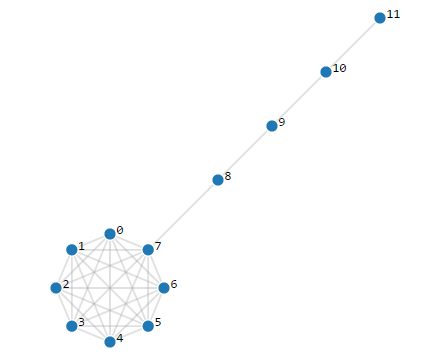
\includegraphics[width=\textwidth]{Lollipop_graph.png}
\caption{Graf lizike (8,4)}
\end{figure}
Oglejmo si, kaj je \textbf{naključni sprehod}. Najprej si izberimo vozlišče $v$ v grafu $G$. Naj bo $d(v)$ število sosedov
 vozlišča $v$. Če začnemo pri $v$, se v naslednjem koraku pomaknem na 
sosednje vozlišče z verjetnostjo $\frac{1}{d(v)}$ in to se nadaljuje tako dolgo kot potrebujemo 
(recimo dokler ne pridemo nazaj v začetno vozlišče ali dokler ne obiščemo vseh vozlišč).

V primeru grafa lizike ima $d(v)$ štiri možne vrednosti. Če se nahajamo na
delu grafu, ki je v obliki poti, imajo vsa vozlišča razen enega dva soseda, in je verjetnost, da
se pomaknemo na naslednjem koraku v sosednje vozlišče $\frac{1}{2}$, oziroma 1, če smo na začetku poti.
V drugem primeru, ko se začetno vozlišče nahaja na polnem grafu, pa je verjetnost enaka $\frac{1}{m-1}$, oziroma
$\frac{1}{m}$, če smo na spoju med kliko in potjo. 

\textbf{Čas pokritja} za vozlišče $u$, označimo z $C_u$, je pričakovani čas oziroma število korakov, da obiščemo vsa vozlišča z začetkom v $u$.
Čas pokritja grafa pa definiramo kot max\{$C_u;u\in V(G)$\}.
\textbf{Čas dosega} za poljubna dva vozlišča $u,v$, označimo z $H_{uv}$, je pričakovani čas oziroma število korakov, da 
pridemo iz vozlišča $u$ v $v$.


\section{Načrt dela}

Za reševanje problema bova uporabila programski jezik Python. Najprej bova napisala funkcije, ki zgenerirajo zahtevan
graf (polni, pot, lizika, malce predelana lizika, ...). Vsaka funkcija sprejme število vozlišč in vrne slovar, čigar
ključi so vozlišča, vrednosti pa seznami sosedov. Nato bova napisala še funkcije naključnih sprehodov, ki kot
vhodni podatek sprejmejo vozlišče, vrnejo pa število korakov, potrebnih za obisk vseh vozlišč, določenega vozlišča
ali vrnitve v začetno vozlišče. Funkcije bodo delovale tako, da bodo na vsakem koraku iz seznama sosedov naključno
izbrale enega. Imela bova še števec korakov in seznam že obiskanih vozlišč, ki nam bo javil, kdaj smo obiskali vsa
vozlišča. Ker gre tu za slučajen sprehod, bova za pričakovano število korakov vzela povprečje večkratnih ponovitev
poskusa. Paziti bova morala tudi, da za začetek sprehoda vzameva primerno vozlišče, saj je čas pokritja definiran kot
najdaljši čas glede na vozlišča v grafu.

\end{document}